%% no need for  \DeclareGraphicsExtensions{.pdf,.eps}

\documentclass[12pt,letterpaper,english]{article}
\usepackage{times}
\usepackage[T1]{fontenc}
\IfFileExists{url.sty}{\usepackage{url}}
                      {\newcommand{\url}{\texttt}}

\usepackage{babel}
%\usepackage{noweb}
\usepackage{Rd}

\usepackage{Sweave}

%\VignetteIndexEntry{Performance Attribution from Bacon}
%\VignetteDepends{PerformanceAnalytics}
%\VignetteKeywords{returns, performance, risk, benchmark, portfolio}
%\VignettePackage{PerformanceAnalytics}

%\documentclass[a4paper]{article}
%\usepackage[noae]{Sweave}
%\usepackage{ucs}
%\usepackage[utf8x]{inputenc}
%\usepackage{amsmath, amsthm, latexsym}
%\usepackage[top=3cm, bottom=3cm, left=2.5cm]{geometry}
%\usepackage{graphicx}
%\usepackage{graphicx, verbatim}
%\usepackage{ucs}
%\usepackage[utf8x]{inputenc}
%\usepackage{amsmath, amsthm, latexsym}
%\usepackage{graphicx}

\title{Autocorrelated Standard Deviation}
\author{R Project for Statistical Computing}

\begin{document}
\Sconcordance{concordance:ACFSTDEV.tex:ACFSTDEV.rnw:%
1 44 1 1 5 1 4 20 1 1 2 1 0 4 1 8 0 1 1 8 0 1 2 1 0 1 2 5 0 1 2 3 1}


\maketitle


\begin{abstract}
The fact that many hedge fund returns exhibit extraordinary levels of serial correlation is now well-known and generally accepted as fact.Because hedge fund strategies have exceptionally high autocorrelations in reported returns and this is taken as evidence of return smoothing, we highlight the effect autocorrelation has on volatility which is hazed by the square root of time rule used in the industry
\end{abstract}



\section{Methodology}
Given a sample of historical returns \((R_1,R_2, . . .,R_T)\),the method assumes the fund manager smooths returns in the following manner, when 't' is the unit time interval:

%Let $X \sim N(0,1)$ and $Y \sim \textrm{Exponential}(\mu)$.  Let
%$Z = \sin(X)$. $\sqrt{X}$.
  
%$\hat{\mu}$ = $\displaystyle\frac{22}{7}$
%e^{2 \mu} = 1
%\begin{equation}
%\left(\sum_{t=1}^{T} R_t/T\right) = \hat{\mu} \\
%\end{equation}
\begin{equation}
 \sigma_{T}  =  T \sqrt{\sigma_{t}} \\
\end{equation}


\section{Usage}

In this example we use edhec database, to compute true Hedge Fund Returns.

\begin{Schunk}
\begin{Sinput}
> library(PerformanceAnalytics)
> data(edhec)
> ACFVol = ACStdDev.annualized(edhec[,1:3])
> Vol = StdDev.annualized(edhec[,1:3])
> Vol
\end{Sinput}
\begin{Soutput}
                              Convertible Arbitrage CTA Global
Annualized Standard Deviation            0.06944619 0.08705599
                              Distressed Securities
Annualized Standard Deviation            0.06355903
\end{Soutput}
\begin{Sinput}
> ACFVol
\end{Sinput}
\begin{Soutput}
                                             Convertible Arbitrage CTA Global
Autocorrelated Annualized Standard Deviation             0.1322706 0.09640755
                                             Distressed Securities
Autocorrelated Annualized Standard Deviation             0.1137627
\end{Soutput}
\begin{Sinput}
> barplot(rbind(ACFVol,Vol), main="ACF and Orignal Volatility",
+          xlab="Fund Type",ylab="Volatilty (in %)", col=c("darkblue","red"), beside=TRUE)
>    legend("topright", c("1","2"), cex=0.6, 
+                    bty="2", fill=c("darkblue","red"));
\end{Sinput}
\end{Schunk}
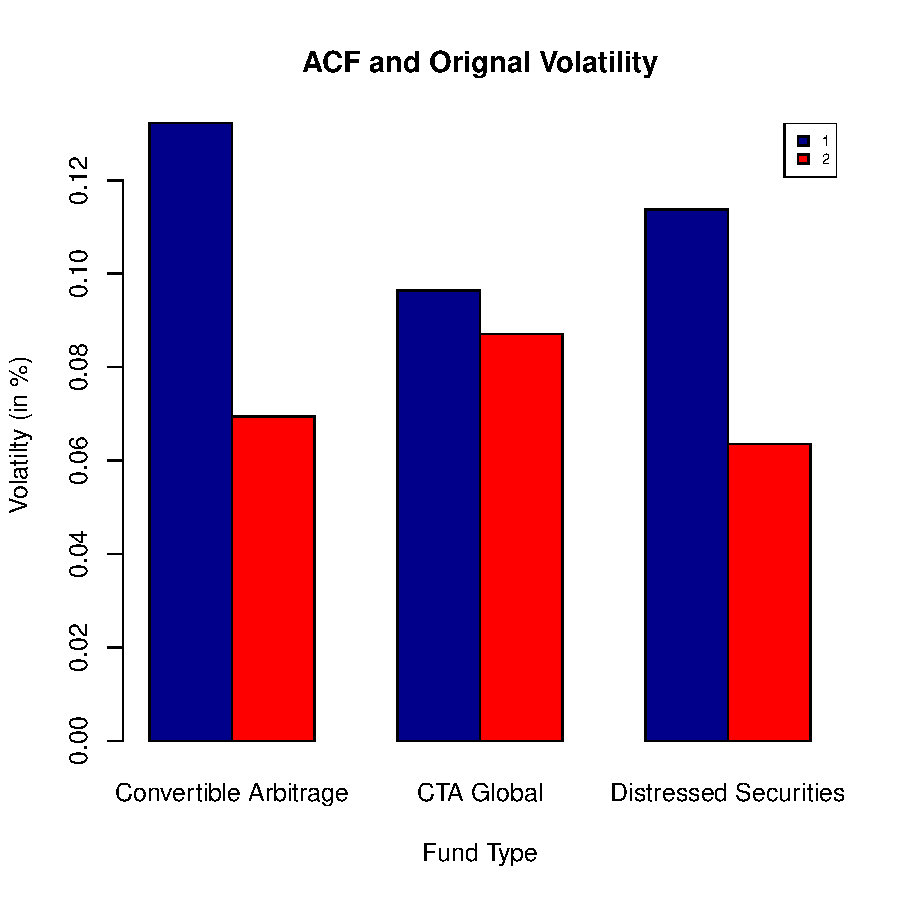
\includegraphics{ACFSTDEV-Graph10}

The above figure shows the behaviour of the distribution tending to a normal IID distribution.For comparitive purpose, one can observe the change in the charateristics of return as compared to the orignal.

\end{document}
